\section{Virtual Analog Synthesis}

Der Begriff "Virtueller Analoger Synthese" wird verwendet, um die Echtzeit-Emulation des analogen Synthesizern der 60er und 70er Jahre zu beschreiben. Die Komplexität und die Ziele einer Emulation können variieren. Einige Emulationen gehen so weit, dass sie die tatsächlichen elektronischen Komponenten der Vintage-Synthese-Schaltungen zu simulieren, andere modellieren nur grob den Signalfluss.

Unabhängig von der Art der Emulation hat virtuell analoger Synthese zwei Probleme mit dem es sich Beschäftigen muss, Latenzzeit und Aliasing. Das Problem der Latenzzeit wurde bereits oben beschrieben. Die Verarbeitung wird eine Verzögerung des Signals erzeugen, die Komplexität der Verarbeitung kann die Verzögerung erhöhen oder mehr CPU-Zyklen verbrauchen. Aliasing ist ein hörbare Verzerrungen des Signals, welches durch Frequenzen verursacht werden die höher sind als die Abtastrate des Systems erlaubt.

Analog-Synthesizer verwenden üblicherweise Subtraktive Synthese. Ein oder mehrere Klangerzeuger ( Oszillatoren ) erzuegen Signale mit besondere harmonische Qualitäten. Diese Signale werden durch Filter geschickt, welche die Frequenzen aus dem Signal "Subtraktieren". Die Oszillatoren, Filter und Amplitude können moduliert werden. Abbildung~\ref{fig:synth_voice_block} ist ein einfaches Blockschaltbild eines typischen Subtraktive Synthesizer Stimme.

\begin{figure}[H]
    \centering
    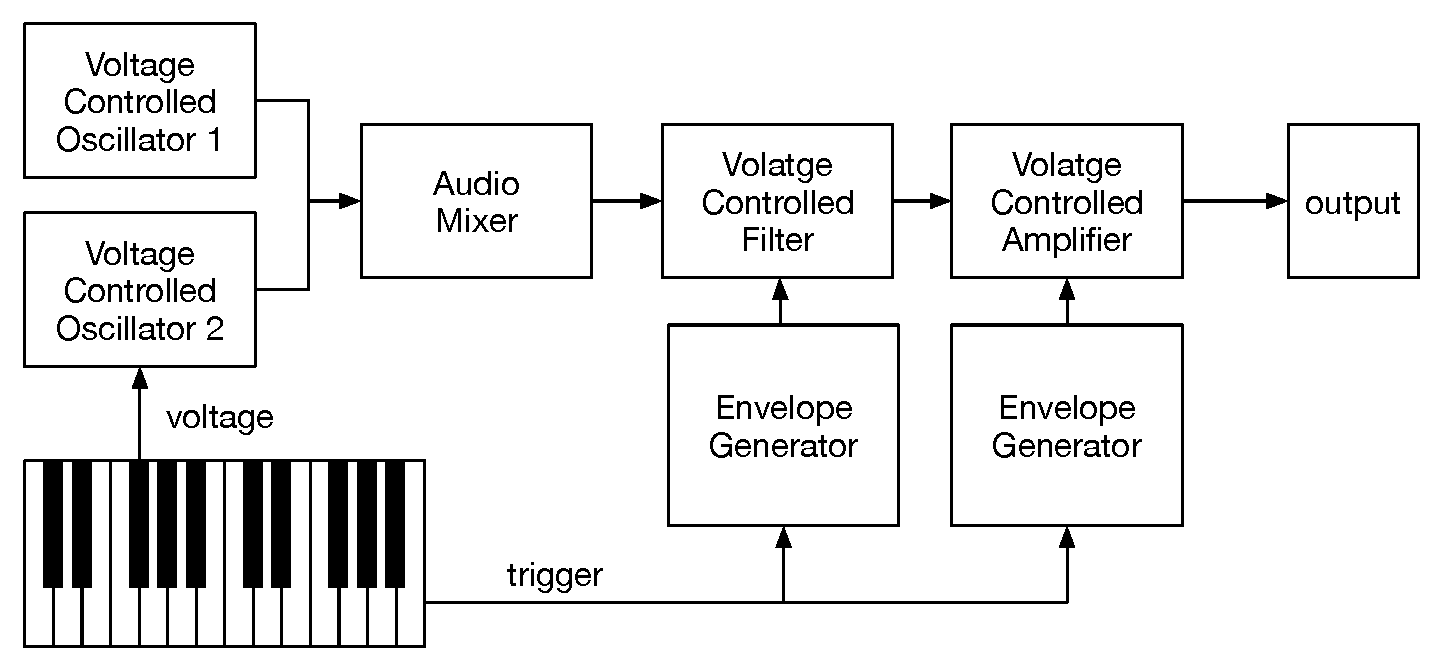
\includegraphics[width=\textwidth]{assets/synth_voice_block.pdf}
    \caption{Blockschaltbild eines Subtraktive Synthesizer Stimme}
    \label{fig:synth_voice_block}
\end{figure}